The rewriting we present is useful in a wide variety of uses cases, with very different execution environments and query characteristics. We distinguish at least four use cases: 1) an ETL framework used for operational intelligence 2) A big data analytics system used by business intelligence users, 3) a web application which provides analytics visuals for a browser and 4) a cloud web service/API for external applications.


\subsection{Operational Intelligence}

Operational Intelligence applications collect machine generated data from logging systems and/or application output for the purposes of monitoring and real-time analytics. It involves two distinct tasks: collecting data, then analyzing it. It is often the case that the database systems used for collection and analysis are distinct, and data must be moved from the former to the latter through the use of ETL tools. 
% 

% Describe query characteristics
It is also often the case that the system used for analysis is a document store such as MongoDB \eat{\jules{find sources which describe why document stores are good for this kind of analysis}}, which stores data as documents with nested structures. One example is clickstream analysis for an online website. To facilitate further analysis, an ETL middleware pre-aggregates daily, hourly and minute hit counts for every web page from a source log file into a target document database using query \ref{list:query2} from appendix \ref{app:examples}. 

\eat{
These stores benefit particularly well from our rewriting, since it targets the queries which are used to produce this nesting.
\begin{figure}[h]
\label{fig:hadoop}
\centering
\caption{Hadoop ETL architecture}
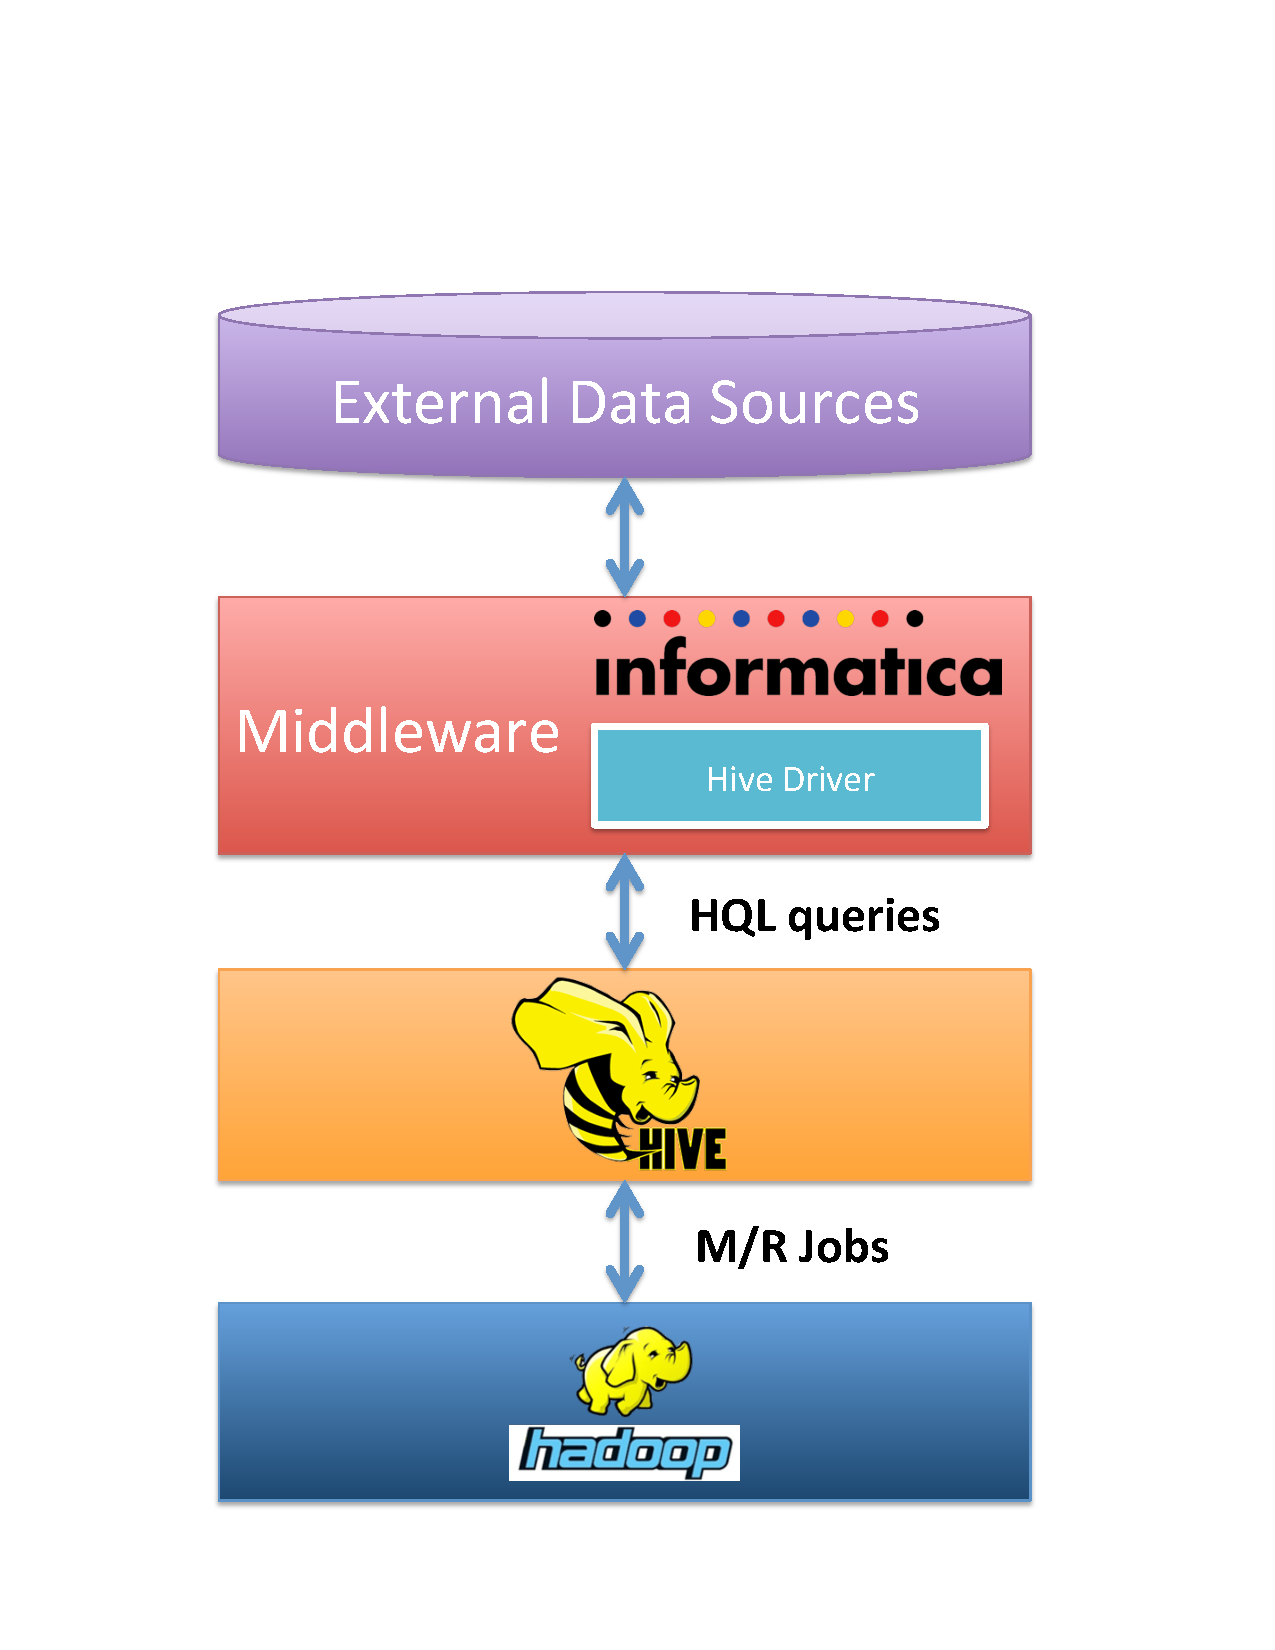
\includegraphics[width=5cm]{images/HadoopETL.pdf}
\end{figure}

% Describe execution environment
On figure \ref{fig:hadoop} is shown the architecture used by Informatica's Big Data Edition product \cite{informaticaBDE}, a commercial ETL middleware with (potentially) access to a Hadoop cluster. In the operational intelligence use case, the ETL tool will move data from a data source (for example a large log file) to a data target such as MongoDB. The middleware possesses its own query processing capabilities, but can delegate a particular processing task to a Hadoop cluster (through Hive) when the data to be processed is too large to fit in the middleware's memory.
}

\subsection{Big Data Analytics System (BDAS)} 

Business intelligence analysts need to make queries for historical and analytical intelligence.  Business intelligence query results are meant to be readable, therefore are small  (a few hundred of rows at most) and typically look at the top-k elements which match a particular criteria. Very fast latencies are not typically a requirement for these kinds of queries, but they sift through very large amounts of data. The number of such queries issued is also expected to be small, given that the number of analysts studying the same dataset at the same time is typically limited.

The execution environment utilized in this use case have typically been parallel data warehouses. However, such systems are inadequate when the result of the formulated queries contain nested collections. For example, consider the following query performed on top of a large retail store dataset: Find the top 30 products that are mostly viewed together with a given an input list of products in an online store \footnote{corresponds to the query 2 from the TPCx-BB benchmark} (query \ref{list:query3} from appendix \ref{app:examples}). For each product in the input list, a collection of 30 products must be found. A new breed of system used when this happens in such cases semi-structured (and parallel) databases, such as AsterixDB.

\eat{
\begin{itemize}
\item Systems built on top of Hadoop (such as Hive) are being used in such cases.
\item Semi-structured parallel query execution engines, such as AsterixDB.
\jules{list might be incomplete}
\end{itemize}

\jules{Should discuss AsterixDB architecture here.}
We argue our rewriting is useful for such BDAS systems with a semi-structured data model. For example, take query \ref{list:query3} from appendix \ref{app:examples}. This query is a typical example of analytical intelligence written by business analysts on a large retail store dataset. Notice that example \ref{list:query3} is exactly an instance of the scenario 4 pattern studied in section 5. 
}

\subsection{Analytics Visualization}

This use case applies to queries issued by analytics/reporting web applications which display nested, aggregated data. Query results for this use case are small enough to be displayed on a computer screen. Moreover, applications tend to have short latency requirements (less than a second) and a large number of users, each requesting multiple distinct visualization renderings as they interact with various UI widgets. As such, visualization queries tend to be numerous and are usually based on small datasets or pre-aggregated data.

For example, consider an analytics web application for a large retail company, which provides its regional and store managers with visuals to help them assess the performance of the clerks working in their store. The application has checkboxes to select clerks working in store $X$, and produces details about the top $K$ largest orders, in terms of total sales price (query \ref{list:query4} from appendix \ref{app:examples}). For each clerk in the selected list, a collection of $K$ orders must be retrieved.

\subsection{Online Web Services \& APIs}

This use cases applies to online web services, typically hosted in the cloud, which provides information to be consumed by external services, such as mobile applications or other web services. Three commercial examples of such services would include:

\begin{itemize}
\item Algolia: a full text search web service, which stores and indexes customer text data (such as product reviews), and provides an API to query it.
\item Keen.IO: a web service which embeds a visual analytics client on the customer's website, and collects/stores the customer data to be visualized.
\item Loggly: a log management web service, which stores and indexes customer logs and allows customers to easily query and visualize them.
\end{itemize}

These web services share a number of characteristics: their queries have typically a low latency requirements, the number of queries answered is large (given each customer can issue an arbitrary number of queries), their APIs only allow a narrow set of highly specialized query patterns and their query results are structured with nesting for program consumption (typically using the JSON data format). Consider a case in which the Loggly web service is used by some large retail website customer. In order to help the customer sift through its page view log, Loggly would provide the per-minute and per-hour page view hit-counts for any given page upon request (query \ref{list:query1} from appendix \ref{app:examples}). The result would produce one tuple per hour, while each minute hit count would be stored in a nested collection field in the corresponding hour tuple. 

